\documentclass{article}
\usepackage[utf8]{inputenc}
\usepackage{graphicx}
\usepackage{float}

\usepackage{listings}
\usepackage{xcolor}
\renewcommand{\figurename}{Figura}
 
\definecolor{codegreen}{rgb}{0,0.6,0}
\definecolor{codegray}{rgb}{0.5,0.5,0.5}
\definecolor{codepurple}{rgb}{0.58,0,0.82}
\definecolor{backcolour}{rgb}{0.95,0.95,0.92}
 
\lstdefinestyle{mystyle}{
    backgroundcolor=\color{backcolour},   
    commentstyle=\color{codegreen},
    keywordstyle=\color{magenta},
    numberstyle=\tiny\color{codegray},
    stringstyle=\color{codepurple},
    basicstyle=\ttfamily\footnotesize,
    breakatwhitespace=false,         
    breaklines=true,                 
    captionpos=b,                    
    keepspaces=true,                 
    numbers=left,                    
    numbersep=5pt,                  
    showspaces=false,                
    showstringspaces=false,
    showtabs=false,                  
    tabsize=2
}
 
\title{Algoritmos y Programaci\'on 1\\
C\'atedra Essaya - Pr\'actica Grace}
\author{Lucas Alejo Pavlov - Legajo 105412}
\date{EJ1 - 2 de septiembre de 2019 - Correctora: Florencia Rodr\'iguez}

\begin{document}

\maketitle

\section*{Parte 1}
\subsection*{Parte 1.1}

\begin{figure}[H]
    \centering
    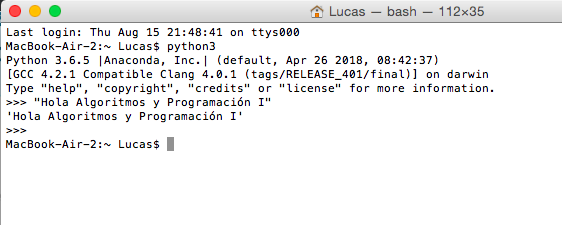
\includegraphics[width=1\textwidth]{parte1-1-cropped.png}
    \caption{Captura de pantalla correspondiente a la parte 1.1.}
    \label{fig:captura-1-1}
\end{figure}

\subsection*{Parte 1.2}
\begin{figure}[H]
    \centering
    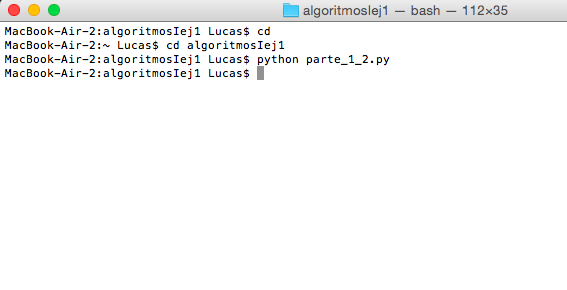
\includegraphics[width=1\textwidth]{parte1-2.png}
    \caption{Captura de pantalla correspondiente a la parte 1.2.}
    \label{fig:captura-1-2}
\end{figure}

\textbf{5)} Para obtener el mismo resultado que en la parte 1.1 deber\'ia usar la funci\'on \texttt{print}, reemplazando la l\'inea
\begin{verbatim}
'Hola Algoritmos y Programación I'
\end{verbatim}
por
\begin{verbatim}
print('Hola Algoritmos y Programación I')
\end{verbatim}

\section*{Parte 2}
\begin{figure}[H]
    \centering
    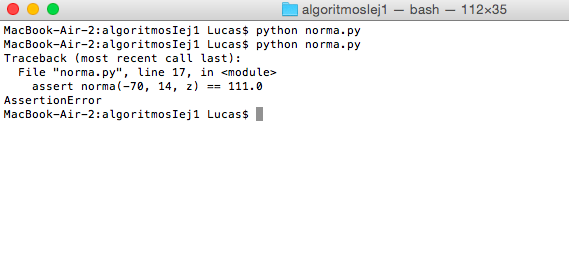
\includegraphics[width=1\textwidth]{parte-2.png}
    \caption{Captura de pantalla correspondiente a la parte 2.}
    \label{fig:captura-2}
\end{figure}

\textbf{4.1)} El programa no tiene ninguna salida salvo que alguno de los asserts sea \texttt{False}. En ese caso la salida es un \texttt{AssertionError} que ocurre en la primera l\'inea en la cual la expresi\'on que se le pasa a \texttt{assert} es \texttt{False}.\\

\noindent
\textbf{4.2)} El error se gener\'o en la l\'inea 17. Significa que la expresi\'on luego de \texttt{assert} en esa l\'inea es \texttt{False} (en el sentido booleano), ya que \texttt{norma(-70, 14, -80)} no es igual a \texttt{111.0}. Para solucionarlo habr\'ia que cambiar esa expresi\'on para que de un resultado verdadero. Se podr\'ia hacer cambiando una o m\'as de las entradas de norma y/o cambiando el resultado de norma, aunque todo hace indicar que la forma que se pide ser\'ia modificando la l\'inea 16, que har\'ia que la entrada de norma que se modifique sea la tercera. Habr\'ia que elegir un valor de \texttt{z} que haga que \texttt{norma(-70, 14, z)} sea igual a \texttt{111.0}. Los valores que hacen eso son $z = 85$ y $z = -85$.\\

\noindent
\textbf{4.3)} En el punto 2 no imprimi\'o nada porque todas las expresiones luego de \texttt{assert} que fueron ejecutadas (es decir, desde la l\'inea 5 hasta la 14, ya que la de la l\'inea 17 estaba comentada) eran \texttt{True}. La instrucci\'on \texttt{assert} no hace nada si lo que est\'a luego de ella es \texttt{True}, en caso contrario (\texttt{False}) termina la ejecuci\'on del programa y sale del mismo devolviendo un error.

\section*{Parte 3}
\begin{figure}[H]
    \centering
    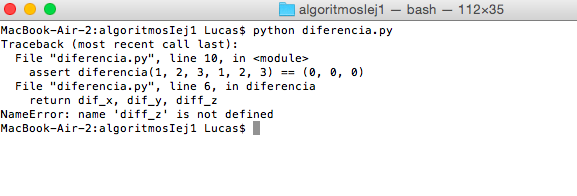
\includegraphics[width=1\textwidth]{parte-3.png}
    \caption{Captura de pantalla correspondiente a la parte 3.}
    \label{fig:captura-3}
\end{figure}

\noindent
\textbf{4)} Se detect\'o un error en la \'ultima l\'inea de la definici\'on de la funci\'on \texttt{diferencia}, ya que se estaba pidiendo devolver una variable que no hab\'ia sido definida anteriormente (\texttt{diff\_z}). Para corregir el error cambi\'e la linea
\begin{lstlisting}[language=Python]
    return dif_x, dif_y, diff_z
\end{lstlisting}
por
\begin{lstlisting}[language=Python]
    return dif_x, dif_y, dif_z
\end{lstlisting}
ya que \texttt{dif\_z} es la variable que fue definida en el cuerpo de la funci\'on. Luego de hacer ese cambio, al correr el programa no sale ning\'un mensaje, con lo cual todas las condiciones planteadas luego de los \texttt{assert} son \texttt{True}.

\section*{Parte 4}

\textbf{4)} Muestra un \texttt{AssertionError} en la l\'inea 10. Luego, si se comenta esa l\'inea, aparece un error en la l\'inea 11, y as\'i sucesivamente, todas las l\'ineas debajo de la 10 dan \texttt{AssertionError}.\\

\noindent
\textbf{5)} Incluyendo llamadas a \texttt{print} en la funci\'on (antes de \texttt{return}) se ve que el problema est\'a en la segunda componente del producto vectorial (\texttt{var2}). Viendo el cuerpo de la funci\'on en esa l\'inea se ve que hay una potenciaci\'on en lugar de una multiplicaci\'on. Corrigiendo ese bug, el programa se ejecuta sin dar ning\'un \texttt{AssertionError}. M\'as espec\'ificamente, hay que cambiar la l\'inea
\begin{lstlisting}[language=Python]
    var2 = z1**x2 - x1*z2
\end{lstlisting}
por
\begin{lstlisting}[language=Python]
    var2 = z1*x2 - x1*z2
\end{lstlisting}

\noindent
\textbf{4.7)}
Si. La l\'inea ser\'ia:
\begin{lstlisting}[language=Python]
    return y1*z2 - z1*y2, z1*x2 - x1*z2, x1*y2 - y1*x2
\end{lstlisting}

\section*{Parte 5}

\textbf{5)} La reutilizaci\'on de funciones es importante ya que permite tener un c\'odigo mucho m\'as ordenado, y hacer un programa por partes puede ahorrarnos tiempo en futuros programas que requieran partes (funciones) similares, es decir, programando las distintas funciones tengo la posibilidad de reutilizarlas m\'as adelante en otros programas ahorrando tiempo.\\

Adem\'as, si alguna funci\'on tiene un bug y se usa muchas veces en un programa, alcanza con corregir la funci\'on para corregir el bug, mientras que si no se escribe el c\'odigo del programa via funciones sino de manera expl\'icita, a la hora de corregir el bug habr\'ia que hacerlo en distintos lugares del c\'odigo, lo cual aumenta el tiempo de trabajo y tambi\'en la probabilidad de saltearse alguna correcci\'on y que el bug persista en alguna instancia del programa final.

\end{document}
